\documentclass[aps,prd,nofootinbib,twocolumn,10pt]{revtex4-2}

\usepackage{amssymb,amsmath,hyperref}
\hypersetup{
	colorlinks=true,
	linktoc=page,
	citecolor=blue,
	linkcolor=blue,
	urlcolor=blue} 
\urlstyle{same}

\usepackage{natbib}

\usepackage{tikz}
\usetikzlibrary{arrows.meta}

\newcommand{\NN}{\mathcal{N}}
\newcommand{\OO}{\mathcal{O}}
\newcommand{\Aa}{\mathcal{A}}
\newcommand{\Tr}{\mathrm{Tr}}

\newcommand{\agl}[2]{\langle#1\, #2 \rangle}
\newcommand{\sqr}[2]{\lbrack #1\, #2 \rbrack}
\newcommand{\tlambda}{\widetilde{\lambda}}

\usepackage[colorinlistoftodos]{todonotes}
\setuptodonotes{color=cyan}
\presetkeys{todonotes}{inline}{}

\begin{document}

%%% --- Frontmatter --- %%%

\title{Generic EFT Operator Basis from 4D Spinor Helicity Formalism}	
\author{Stefano De Angelis}
\email{s.deangelis@qmul.ac.uk}
\affiliation{Centre for Theoretical Physics, School of Physics and Astronomy, Queen Mary University of London, Mile End Road, London E1 4NS, United Kingdom}
\date{\today} 
\begin{abstract}
     Something
\end{abstract}
	
	
% \maketitle
	
\tableofcontents

\listoftodos

% \section{Introduction}

\section{Operators and Minimal Amplitudes}

\todo{three-points are special, we do only four points - no special kinematics involved}

Each effective interaction will be identified by its {\it minimal} amplitude, {\it i.e.} the amplitude at leading order which does not vanish in free theory (if we switch off all the other interactions). This has to be a contact term, {\it i.e.} there are no intermediate modes propagating.

As a first step in the classification procedure, we fix the mass-dimension $\left[\mathcal{O}\right]$ of the marginal operators for which we want to find a complete basis. From the minimal amplitudes we strip off the coupling of the effective interaction, which is related to the dimension of the corresponding marginal operator by
\begin{equation}
    \left[g_{\mathcal{O}}\right] = 4-\left[\mathcal{O}\right]\ .
\end{equation}
What we are looking for are the kinematic structures which have mass dimension
\begin{equation}
\label{eq::dimcontact}
    \left[\mathcal{O}\right]-n\geq 0\ ,
\end{equation}
where $n$ is the number of external legs in the corresponding minimal amplitude. Equation \eqref{eq::dimcontact} provides a constraint on $n$ which can be further refined by taking into account which types of particles are found in the amplitudes. In fact, in order to get helicity weights right, each vector in the minimal amplitude will contribute at least with two spinor variables and each fermion at least with one. This leads to the stronger constraint. This condition is not only necessary but also sufficient for having local interactions.
\begin{equation}
\label{eq::particleconstraint}
 \left[\mathcal{O}\right] - n \geq \frac{1}{2} \cdot \left( 2\, n_g + n_f \right) \, \hspace{0.2em} \implies \hspace{0.2em} 2 n_g + \frac{3}{2} n_f + n_s \leq \left[\mathcal{O}\right]\ ,
\end{equation}
where $n_g$, $n_f$ and $n_s$ are respectively the number of vectors, fermions and scalars and clearly $n=n_g+n_f+n_s$.
Next, we need to take into account the constraints coming from the condition that our kinematic structures must be ${\rm SL}(2,\mathbb{C})$ invariant. This requires to further distinguish between helicities of the different particles, and to find all the $(n_{g^-},n_{g^+},n_{f^-},n_{f^+},n_s)$. The superscript of the subscript specify the helicity of the particles: $n_g = n_{g^-}+n_{g^+}$ and  $n_f = n_{f^-}+n_{f^+}$. compatible with the constraint \eqref{eq::particleconstraint}.
Once $n_g$, $n_f$ and $n_s$ are fixed, we take into account that every state can contribute to the kinematic structures with powers of its momentum, which correspond to derivates in the operator language. The total number of momenta $n_\partial$ is fixed by saturating the mass dimension constraint to
\begin{equation}
    n_\partial = \left[ \mathcal{O}\right] - 2 n_g - \frac{3}{2}n_f - n_s \> .
\end{equation}

\section{The massless basis}

In this section we are going to extend the on-shell methods to the classification of effective interactions \cite{Shadmi:2018xan,Falkowski:2019zdo,Durieux:2020gip} in the SMEFT \cite{Ma:2019gtx,Aoude:2019tzn,Durieux:2019eor,Durieux:2019siw}, corresponding in the Lagrangian formalism to insertions of marginal operators \cite{Grzadkowski:2010es,Lehman:2014jma,Murphy:2020rsh,Liao:2020jmn}. First we are going to classify all the independent kinematic structures in a generic theory in four dimensions introducing a new algorithm in terms of graphs and then we will consider the specific case of the Standard Model, combining these with the colour structures.

\subsection{Kinematic structures from spinor helicity variables}\label{sec:kinematics}
%
A simple way of finding all the possible structures is to identify them with an oriented multigraph, where each vertex is associated to a particle, and the edges correspond to angle (red) or square (blue) ${\rm SL}(2,\mathbb{C})$ invariants. The orientation of the edges then keeps track of the ordering of particles in the brackets and thus provides potential minus signs.

The valence of each vertex is given by two natural numbers $v^{i}=(v^i_a,v^{i}_s)$ such that $v^i_s-v^i_a =2 h_i$ is the helicity of the $i^{\rm th}$ particle (see, for example, Figure~\ref{fig:2graphexample}). Finally, for reasons which will become clear in the next section, we consider a circular embedding for our graphs, in other words we take all the nodes to be  ordered points on a circle.
This method has proven to be a computationally efficient way of finding a basis of independent structures up to Schouten and momentum conservation identities. %In particular, the former act separately on angle and square invariants, while the latter mixes the two structures. We are going to show how to deal with this identities in terms of above mentioned multigraphs.
Notice that the former act separately on angle and square invariants, while the latter mixes the two structures. In the following sections we are going to show how to deal with these identities in terms of above mentioned multigraphs.

\begin{figure}[!ht]
    \label{fig::multigraphEx}
	    \begin{center}
		    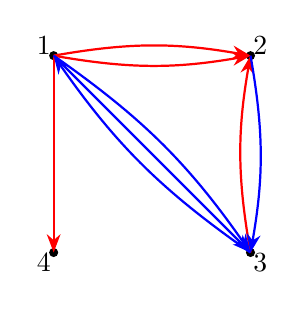
\begin{tikzpicture}[scale=2.5,>=Stealth]
		    
			    \node at (-0.05,-0.05) {$4$};
			    \node at (-0.05,1.05) {$1$};
			    \node at (1.05,1.05) {$2$};
			    \node at (1.05,-0.05) {$3$};
			    
			    \draw [fill] (0,0) circle [radius = 0.02];
			    \draw [fill] (1,0) circle [radius = 0.02];
			    \draw [fill] (0,1) circle [radius = 0.02];
			    \draw [fill] (1,1) circle [radius = 0.02];
			    
			    \draw [<-,thick,red](0,0) -- (0,1);
			    
			    \draw [->,thick,red](0,1) to [out=-10,in=-170] (1,1);
			    \draw [->,thick,red](0,1) to [out=10,in=-190] (1,1);
			    
			    \draw [<-,thick,red](1,1) to [out=-100,in=100] (1,0);
			    \draw [->,thick,blue](1,1) to [out=-80,in=80] (1,0);
			    
			    \draw [->,thick,blue](0,1) -- (1,0);
			    \draw [<-,thick,blue](0,1) to [out=-55,in=145] (1,0);
			    \draw [->,thick,blue](0,1) to [out=-35,in=125] (1,0);
	
		    \end{tikzpicture}
            \hspace{1cm}
	        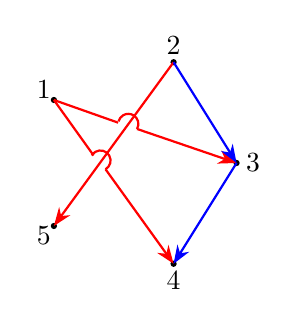
\begin{tikzpicture}[scale=1.6,>=Stealth]
	            
	            \node at (-0.08,-0.08) {$5$};
			    \node at (-0.08,1.08) {$1$};
			    \node at (0.95,1.43) {$2$};
			    \node at (1.58,0.5) {$3$};
			    \node at (0.95,-0.43) {$4$};
			    
			    \draw [fill] (0,0) circle [radius = 0.02];
			    \draw [fill] (0,1) circle [radius = 0.02];
			    \draw [fill] (0.95,1.3) circle [radius = 0.02];
			    \draw [fill] (1.45,0.5) circle [radius = 0.02];
			    \draw [fill] (0.95,-0.3) circle [radius = 0.02];
			    
			    %\draw [->,thick,red](0,1) -- (1.45,0.5);
			    %\draw [->,thick,red](0,1) -- (0.95,-0.3);
			    \draw [->,thick,red](0.95,1.3) -- (0,0);
			    
			    \draw [->,thick,red](0.41,0.45) -- (0.95,-0.3);
			    \draw [thick,red](0,1) -- (0.315,0.56);
			    \draw [thick,red] (0.41,0.45) arc (-60:150:0.08);
			    %\draw [fill] (0.315,0.56) circle [radius = 0.02];
			    %\draw [fill] (0.41,0.45) circle [radius = 0.02];
			    %\draw [fill] (0.66,0.77) circle [radius = 0.02];
			    %\draw [fill] (0.51,0.82) circle [radius = 0.02];
			    \draw [->,thick,red](0.66,0.77) -- (1.45,0.5);
			    \draw [thick,red](0,1) -- (0.51,0.82);
			    \draw [thick,red] (0.66,0.77) arc (-30:165:0.08);
			    
			    \draw [->,thick,blue](0.95,1.3) -- (1.45,0.5);
			    \draw [->,thick,blue](1.45,0.5) -- (0.95,-0.3);
	            
	        \end{tikzpicture}
	    \end{center}
    \caption{The graph associate to the kinematic structures $\textcolor{red}{\agl{1}{2}^2 \agl{1}{4} \agl{3}{2}} \textcolor{blue}{\sqr{2}{3}\sqr{1}{3}^2 \sqr{3}{1}}$ and $\textcolor{red}{\agl{1}{3} \agl{1}{4} \agl{2}{5}} \textcolor{blue}{\sqr{2}{3}\sqr{3}{4}}$ respectively.}
	\label{fig:2graphexample}
\end{figure}

\subsubsection{Schouten identities}

Schouten identities for angle and square brackets read
\begin{equation}\label{eq:Schouten}
\begin{aligned}
    \agl{1}{2}\agl{3}{4} + \agl{2}{3}\agl{1}{4} + \agl{3}{1}\agl{2}{4} &= 0\ ,\\
    \sqr{1}{2}\sqr{3}{4} + \sqr{2}{3}\sqr{1}{4} + \sqr{3}{1}\sqr{2}{4} &= 0\ .
\end{aligned}
\end{equation}

Thinking of the kinematic structures in terms of graphs, specifically using the already mentioned circular embedding, one way of implementing \eqref{eq:Schouten} is by untying crossing edges as shown in Figure \ref{fig::Schouten}. In a generic graph, this can be applied recursively until, after a finite number of steps, we end up with graphs which do not have any crossing. It is then clear that a basis of kinematic structures which are independent under Schouten identities can be obtained by building a basis of planar graphs only.

\begin{figure}[!ht]
    \begin{center}
		    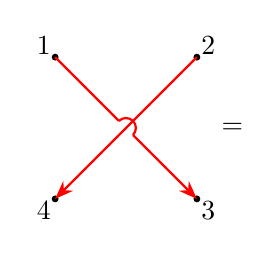
\begin{tikzpicture}[scale=1.8,>=Stealth]
		    
			    \node at (-0.08,-0.08) {$4$};
			    \node at (-0.08,1.08) {$1$};
			    \node at (1.08,1.08) {$2$};
			    \node at (1.08,-0.08) {$3$};
			    \node at (1.25,0.5) {$=$};
			    
			    \draw [fill] (0,0) circle [radius = 0.02];
			    \draw [fill] (1,0) circle [radius = 0.02];
			    \draw [fill] (0,1) circle [radius = 0.02];
			    \draw [fill] (1,1) circle [radius = 0.02];
			    
			    \draw (1,0) [<-,thick,red] -- (0.55,0.45);
			    \draw [thick, red] (0.45,0.55) arc (135:-45:0.07);
			    \draw [thick, red] (0.45,0.55) -- (0,1);
			    \draw [->,thick,red](1,1) -- (0,0);
	
		    \end{tikzpicture}
		    \begin{tikzpicture}[scale=1.8,>=Stealth]
		    
			    \node at (-0.08,-0.08) {$4$};
			    \node at (-0.08,1.08) {$1$};
			    \node at (1.08,1.08) {$2$};
			    \node at (1.08,-0.08) {$3$};
			    \node at (1.25,0.5) {$+$};
			    
			    \draw [fill] (0,0) circle [radius = 0.02];
			    \draw [fill] (1,0) circle [radius = 0.02];
			    \draw [fill] (0,1) circle [radius = 0.02];
			    \draw [fill] (1,1) circle [radius = 0.02];
			    
			    \draw [<-,thick,red](1,0) -- (1,1);
			    \draw [->,thick,red](0,1) -- (0,0);
	
		    \end{tikzpicture}
		    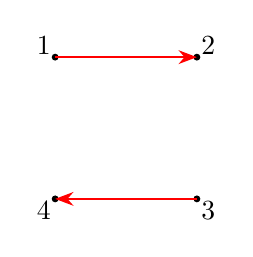
\begin{tikzpicture}[scale=1.8,>=Stealth]
		    
			    \node at (-0.08,-0.08) {$4$};
			    \node at (-0.08,1.08) {$1$};
			    \node at (1.08,1.08) {$2$};
			    \node at (1.08,-0.08) {$3$};
			    
			    \draw [fill] (0,0) circle [radius = 0.02];
			    \draw [fill] (1,0) circle [radius = 0.02];
			    \draw [fill] (0,1) circle [radius = 0.02];
			    \draw [fill] (1,1) circle [radius = 0.02];
			    
			    \draw [->,thick,red](0,1) -- (1,1);
			    \draw [->,thick,red](1,0) -- (0,0);
	
		    \end{tikzpicture}
		\end{center}
	\caption{Schouten identities are equivalent to untying crossings for both the two graphs in the multigraph: $\textcolor{red}{\agl{1}{3}\agl{2}{4}} = \textcolor{red}{\agl{1}{4}\agl{2}{3}} + \textcolor{red}{\agl{1}{2}\agl{3}{4}}$.}
    \label{fig::Schouten}
\end{figure}

\todo{the adjacency matrix, planarity conditions and schouten and antissymmetry of the brackets}

\subsubsection{Momentum conservation}

In general, we consider an $n$-point amplitude with $n_\partial > 0$. Each momentum in the amplitude can be assigned to any of the $n$ particles, which increases the valence of the corresponding vertex by $(1,1)$. The number of momenta associated to each vertex is then $\min\{v^i_a,v^i_s\}$.

We can take into account most of the relations coming from momentum conservation just by excluding the momentum of the $n^{\rm th}$-particle from the previous assignment. Then the $n^{\rm th}$-vertex will have valence $(\frac{|h_n|+h_n}{2},\frac{|h_n|-h_n}{2})$.

There are however $n$. One of which can be written as a linear combination of the other $n-1$. additional relations coming from momentum conservation which do not explicitly involve the momentum of the $n^{\rm th}$-particle:
\begin{align}
\label{eq::momcons2}
    0 = 
    \begin{cases}
        \sum\limits_{j=1}^{n-1} \agl{i}{j} \sqr{j}{n} &  h_n>0\\[.5em]
        \sum\limits_{j=1}^{n-1} \agl{n}{j} \sqr{j}{i} &  h_n<0\\
    \end{cases}
\end{align}
which are a consequence of the Dirac equation $p_{n\, \alpha \dot{\alpha}}\, \tlambda_{n}^{\dot{\alpha}}=\, 0 \, = \lambda^{\alpha}_n\, p_{n\, \alpha \dot{\alpha}}$, and
\begin{equation}
\label{eq::momcons1}
    \sum_{i=1}^{n-2} \sum_{j=i+1}^{n-1} s_{i j} = 0\ ,\\
\end{equation}
Some observations are in order:
\begin{itemize}
    \item The Schouten identities do not change the valences of vertices in the multigraph, so they do not change the number of momenta associated to each vertex.
    %\item Since We want a basis of planar graphs, we solve most of the \eqref{eq::momcons2} for one of the momenta which maximises the number of planar multigraphs, the natural choice being either $p_1$ or $p_{n-1}$ (a different choice would give an over-counting of the independent structures) . Most of the relations in \eqref{eq::momcons2} are taken into account discarding all the structures with $\agl{i}{n-1} \sqr{n-1}{n}$ or $\agl{n}{n-1} \sqr{n-1}{i}$ according to the helicity of the $n^{\rm th}$-particle (or equivalently $\agl{i}{1} \sqr{1}{n} \big/ \agl{n}{1} \sqr{1}{i}$).
    %\item Among \eqref{eq::momcons2}, there is one relation which do not involve neither $p_n$ nor $p_{n-1}$. This is taken into account discarding those structures where $\agl{n-1}{1} \sqr{1}{n} \big/ \agl{n}{1} \sqr{1}{n-1}$ appears (or $\agl{1}{n-1} \sqr{n-1}{n} \big/ \agl{n}{n-1} \sqr{n-1}{1}$).
    \item Since we want a basis of planar graphs, we solve all but one of the \eqref{eq::momcons2} for one of the momenta which maximises the number of planar multigraphs, the natural choice being either $p_1$ or $p_{n-1}$ (a different choice would give an over-counting of the independent structures). The considered identities are then taken into account by simply discarding all the structures involving $\agl{i}{n-1} \sqr{n-1}{n}$ or $\agl{n}{n-1} \sqr{n-1}{i}$ according to the helicity of the $n^{\rm th}$-particle (or equivalently $\agl{i}{1} \sqr{1}{n} \big/ \agl{n}{1} \sqr{1}{i}$).
    \item Among \eqref{eq::momcons2}, there is one relation which does not involve neither $p_n$ nor $p_{n-1}$. This is taken into account by discarding those structures where $\agl{n-1}{1} \sqr{1}{n} \big/ \agl{n}{1} \sqr{1}{n-1}$ appears (or $\agl{1}{n-1} \sqr{n-1}{n} \big/ \agl{n}{n-1} \sqr{n-1}{1}$).
    \item Finally, the constraint \eqref{eq::momcons1} forces us to discard the terms proportional to $s_{1\, n-1}$.
\end{itemize}
This algorithm classifies efficiently all the ${\rm SL}(2,\mathbb{C})$-invariant structures which are polynomial in the spinor variables with fixed mass dimension and helicity configuration, associated to each $(n_{g^-},n_{g^+},n_{f^-},n_{f^+},n_s)$. It also provides a very simple way of writing the dependent structures as linear combinations of the independent ones. We also notice that this algorithm an be applied also beyond gauge theories. Furthermore, the generalisation of this algorithm to massive spinors is possible and it will be discussed in future works.

\section{The massive basis}

The classification of independent structures in massive theories involves more technical considerations, but it is doable from a generalisation presented above for fully massless theories. The sources of such additional complications are two:
\begin{enumerate}
	\item The little group structures
	\item The equations of motion
\end{enumerate}
\todo{simplifications massive states as irreducible representation of LG}
With respect to the massless case, we have additional Schouten identities to take into account for the LG indices.
\begin{itemize}
	\item \textbf{Schouten identities for Lorentz} are taken into account by considering planar graphs. The linear relations are easily found by iteratively untying the crossing. In the massive case, this procedure does not distinguish between massive spinor with contracted and free LG indices.
	\item \textbf{Schouten identities for LG} can involve either a momentum and a spinor with free LG index $p_{i \alpha \dot{\alpha}}\, \widetilde{\lambda}^I_{i \dot{\beta}}$ or $p_{i \alpha \dot{\alpha}}\, \lambda^I_{i \beta}$ or two momenta $p_{i \alpha \dot{\alpha}}\, p_{i \beta \dot{\beta}}$.
	\begin{enumerate}
		\item The latter tells us that we have to associate different vertices in the graph to momenta and free indices spinor (whose LG indices are symmetrised). Schouten identities will be again equivalent to untying crossings:
		\begin{equation}
			p_{i \alpha \dot{\alpha}}\, \widetilde{\lambda}^I_{i \dot{\beta}} = p_{i \alpha \dot{\beta}}\, \widetilde{\lambda}^I_{i \dot{\alpha}} + \epsilon_{\dot{\alpha} \dot{\beta}} p_{i \alpha \dot{\gamma}}\, \widetilde{\lambda}^{I \dot{\gamma}}_{i}
		\end{equation}
		or, equivalently, for the “undotted” spinors.
		\item The former tells us that each momenta must be mapped into an new vertex (with a single red and a single blue edge on the vertex). Again we see that Schouten is equivalent to untying the crossing between lines of the same type:
		\begin{equation}
			p_{i \alpha \dot{\alpha}} p_{i \beta \dot{\beta}} = p_{i \beta \dot{\alpha}} p_{i \alpha \dot{\beta}} + \epsilon_{\alpha \beta} p_{i \alpha \dot{\gamma}} p_{i \beta}^{\dot{\gamma}}
		\end{equation}
		or, equivalently, for the “dotted” indices.
	\end{enumerate}
	Then we find a proliferation of vertices, each particle is associated to a vertex carrying both helicity weight and momenta for massless particles and only spin weight for massive one. For each insertion of massive momenta we need to add a vertex next to the spin vertex of the corresponding particle.
	\item \textbf{Momentum conservation} is now taken identically with respect to the massless case:
	
	which is not a great manipulation of graphs, but we take systematically.
\end{itemize}
These are the operations on graph to find a basis of contact terms.

The $m_i^2$-terms must be eliminated. From a graphic point of view these terms correspond to two momentum vertices of the same massive particle connected by both the red and the blue edge.

Terms proportional to $p_i |\mathbf{i}] = m_i |\mathbf{i}]$ or $\langle \mathbf{i}| p_i = m_i \langle \mathbf{i}|$ should or should not be eliminated according to the spin of the associate particle. From a graphical point of view, they correspond to a momentum vertex connected to the corresponding spin vertex by an (blue or red) edge.
\begin{itemize}
	\item If $s_i< 1$ then we must eliminate them as they correspond to lower dimension operators multiplied with $m_i$ factor.
	\item If $s_i= 1$ and the spin-vertex is connected to a single momentum vertex by only one edge (either blue or red), then we can keep this term. The reason for this is that we have for any $|\mathbf{i}]\langle \mathbf{i}|$ we have an inverse power of the mass $m_i$ from the polarisation tensor.
	\item If $s_i= 1$ and we have multiple edges of this type, then we eliminate the graph.
\end{itemize}
This method should provide both a contact-term basis and a systematic way of finding all the linear relations between different terms.

% \begin{acknowledgments}
%     SDA is a
% \end{acknowledgments} 
    
\appendix

\section{The spinor helicity formalism: review and conventions}
\label{sec:spinorhelicity}

\section{Rational Kinematics and Massive Momentum Twistors}
    \label{sec:massivetwistors}

\bibliographystyle{JHEP}
\bibliography{papers}

\end{document}

% \documentclass[10pt]{article}

% \usepackage[inner=2cm,outer=2cm,top=2cm,bottom=2cm]{geometry}
% \usepackage[tiny]{titlesec}

% \usepackage{multicol}
% \usepackage{amssymb}

% \begin{document}

% \begin{center}
%     {
%         \Large
%         \textbf{Generic EFT Operator Basis from 4D Spinor Helicity Formalism}
%     } 
% \end{center}

% \begin{center}
%     Stefano De Angelis\\[.35em]
%     \textit{
%         \footnotesize Centre for Theoretical Physics, 
%         School of Physics and Astronomy\\
%         Queen Mary University of London,
%         Mile End Road, London E1 4NS, United Kingdom
%     }
% \end{center}


% \begin{abstract}
%     \noindent hello
% \end{abstract}

% \begin{multicols}{2}
% \section{Introduction}
%     hello
% \end{multicols}

% \end{document}